\section{E. Even하게 익은 스테이크}

\begin{frame} % No title at first slide
    \sectiontitle{E}{Even하게 익은 스테이크}
    \sectionmeta{
        출제자 -- 노태윤(\consolas{\href{https://solved.ac/profile/areian13}{@areian13}})\\
        태그: \consolas {\#binary\_search, \#parametric\_search}\\
        예상 난이도 -- \textbf{\color{acS1}Silver1}
    }
    \begin{itemize}
        \item 제출 60번, 정답 5명 (정답률 8.3\%)
        \item 처음 푼 사람: 김0원 48분
    \end{itemize}
\end{frame}
%----------------------------------------------------------------------------
\begin{frame}{\textbf{E}. Even하게 익은 스테이크}
    \begin{itemize}
        \item 화력이 $f$일 때, 스테이크를 모두 굽는 시간  
        $\texttt{total\_time}(f)=\sum_{i=1}^{n}\left\lceil \frac{s_i}{f} \right\rceil$이고,\\
        우리의 목표는 $\texttt{total\_time}(f) \le t$인 최소 정수 $f$를 찾는 것입니다.
        \item 참고로 $\lceil \, \rceil$은 올림이란 뜻으로 $\lceil 0.0...01 \rceil=1$입니다.\\
        따라서 화력을 무한하게 올리더라도  $\texttt{total\_time}(\infty)=\sum_{i=1}^{n}\left\lceil 0^+ \right\rceil=n$이므로,\\
        $t<n$인 경우 $t$분 이내에 모든 스테이크를 굽는 것은 불가능하여\\
        이때 -1을 출력하면 됩니다.

        \item 추가로 모든 $i$에 대해 $\left\lceil \frac{s_i}{\max(s)}=1 \right\rceil$이므로 $\max(s)$ 이상의 화력은 의미가 없습니다.

    \end{itemize}
\end{frame}
%----------------------------------------------------------------------------
\begin{frame}{\textbf{E}. Even하게 익은 스테이크}
    \begin{itemize}
        \item 직관적으로 $f$가 증가함에 따라 $\texttt{total\_time}(f)$는 단조 감소하는 그래프임을 알 수 있습니다.\\
        한국말로 풀어쓰면, 화력이 세지면 굽는 시간이 줄어든다는 말입니다.

        \bigskip

        \begin{center}
            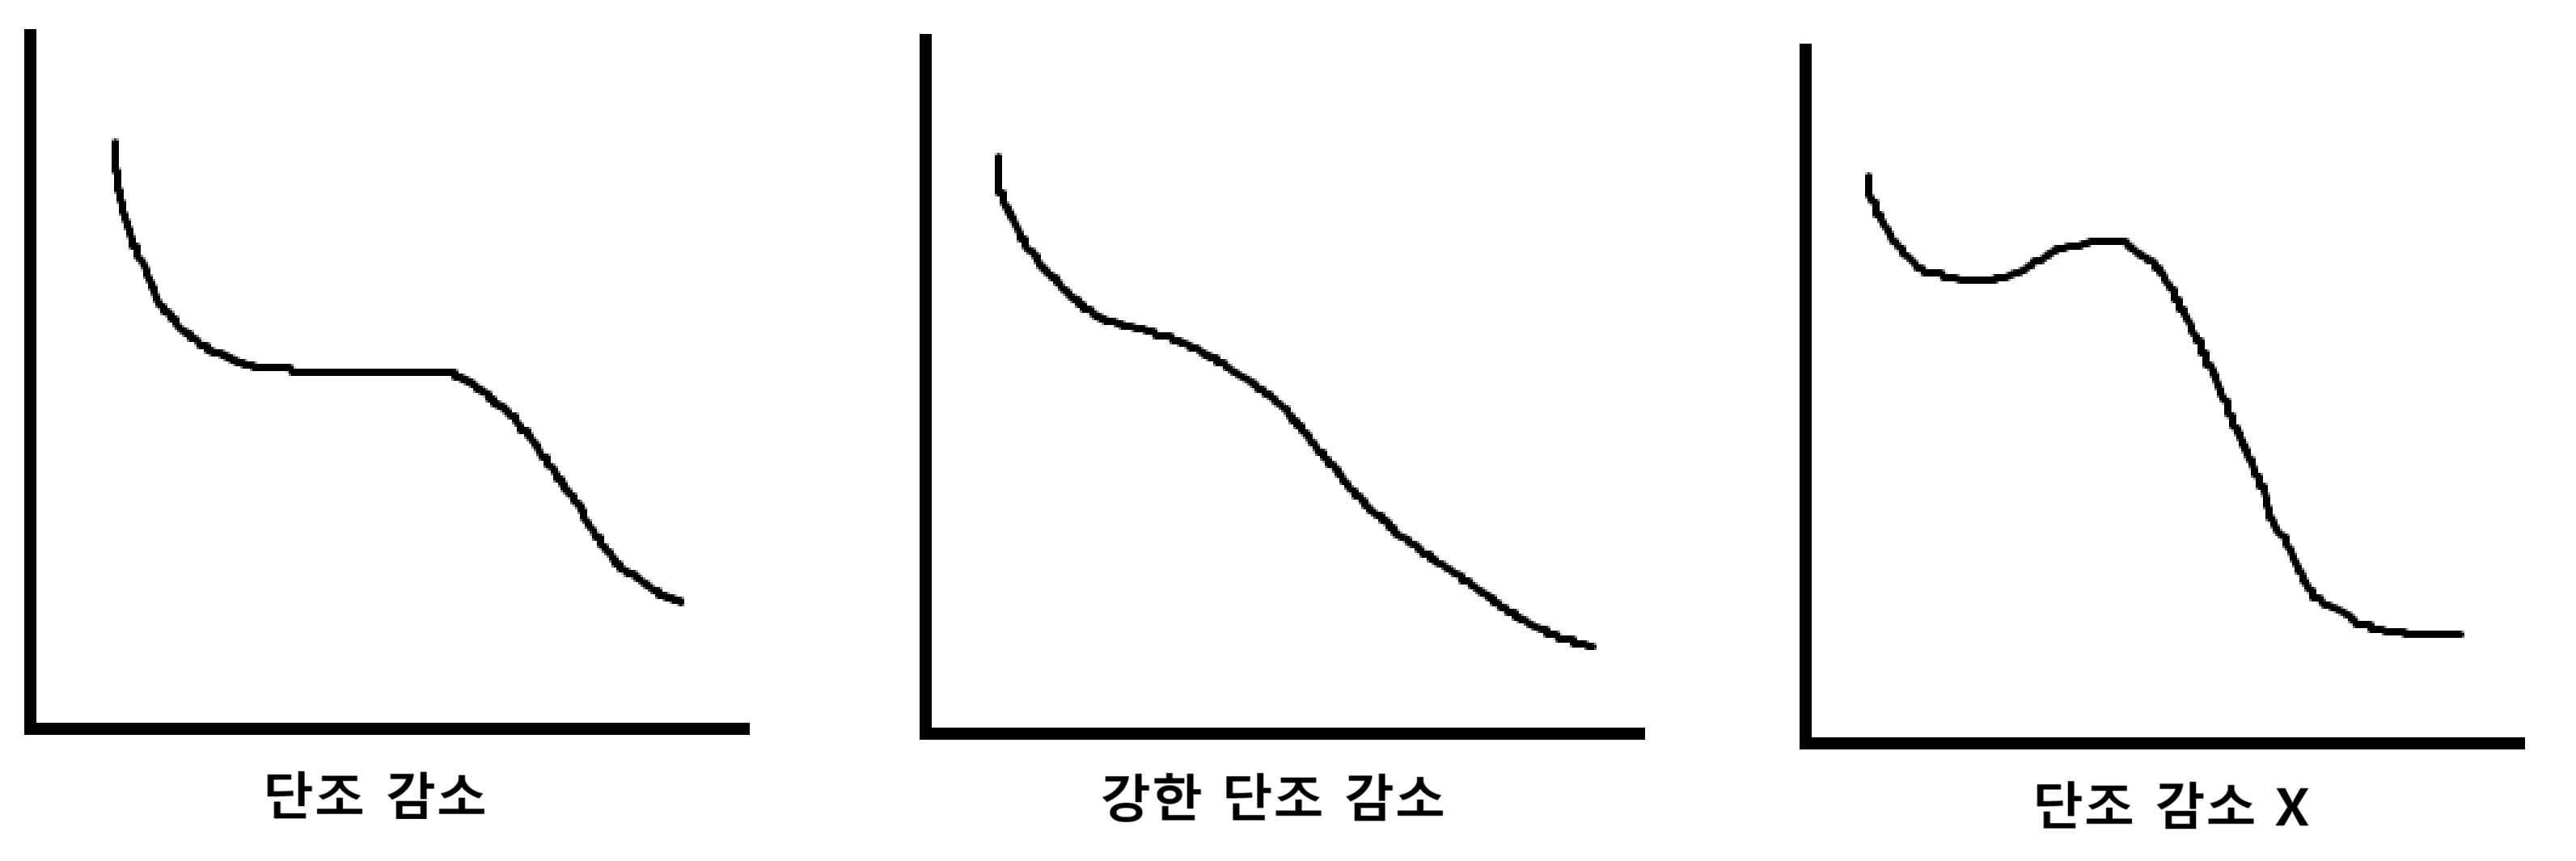
\includegraphics[width=0.9\linewidth]{images/monoton.png}
        \end{center}
    \end{itemize}
\end{frame}
%----------------------------------------------------------------------------
\begin{frame}{\textbf{E}. Even하게 익은 스테이크}
    \begin{itemize}
        \item 배열 혹은 함수가 단조 감소, 단조 증가한다면 이분 탐색을 사용할 수 있습니다.\\
        탐색 범위 $\texttt{start}=1, \texttt{end}=\max(s)$겠네요.\\
        입력 조건산 $s_i$는 최대 $10^9$이니, $\texttt{end}=10^9$으로 해도 됩니다.\\
        이렇게 범위를 잡은 후에 이분 탐색을 해주면 됩니다.

        \item 시간 복잡도\\
        이분 탐색으로 $f$를 결정하는 비용 = $O(\log 10^9)$\\
        $\texttt{total\_time}(f)$ 를 계산하는 비용 = $O(n)$\\
        이 둘을 곱한 $O(n \log 10^9)$
    \end{itemize}
\end{frame}